\section{Figures}
\begin{figure}
    \centering
    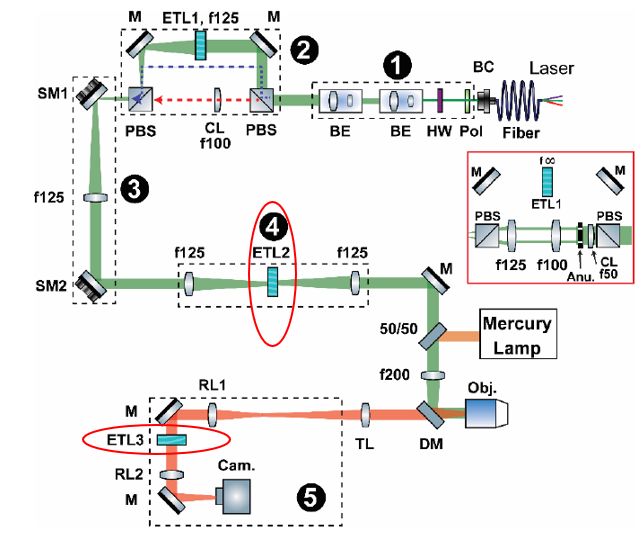
\includegraphics[scale=.50]{system.png}
    \caption[]{This figure, adapted from Liu et al \cite{Liu} with the permission of the corresponding author, depicts the optical design of our system. The ETLs used for remote focusing (circled in red) are at the focal planes of the 4F system, which are conjugate to the back focal plane of the objective.}
\end{figure}
\begin{figure}
    \centering
    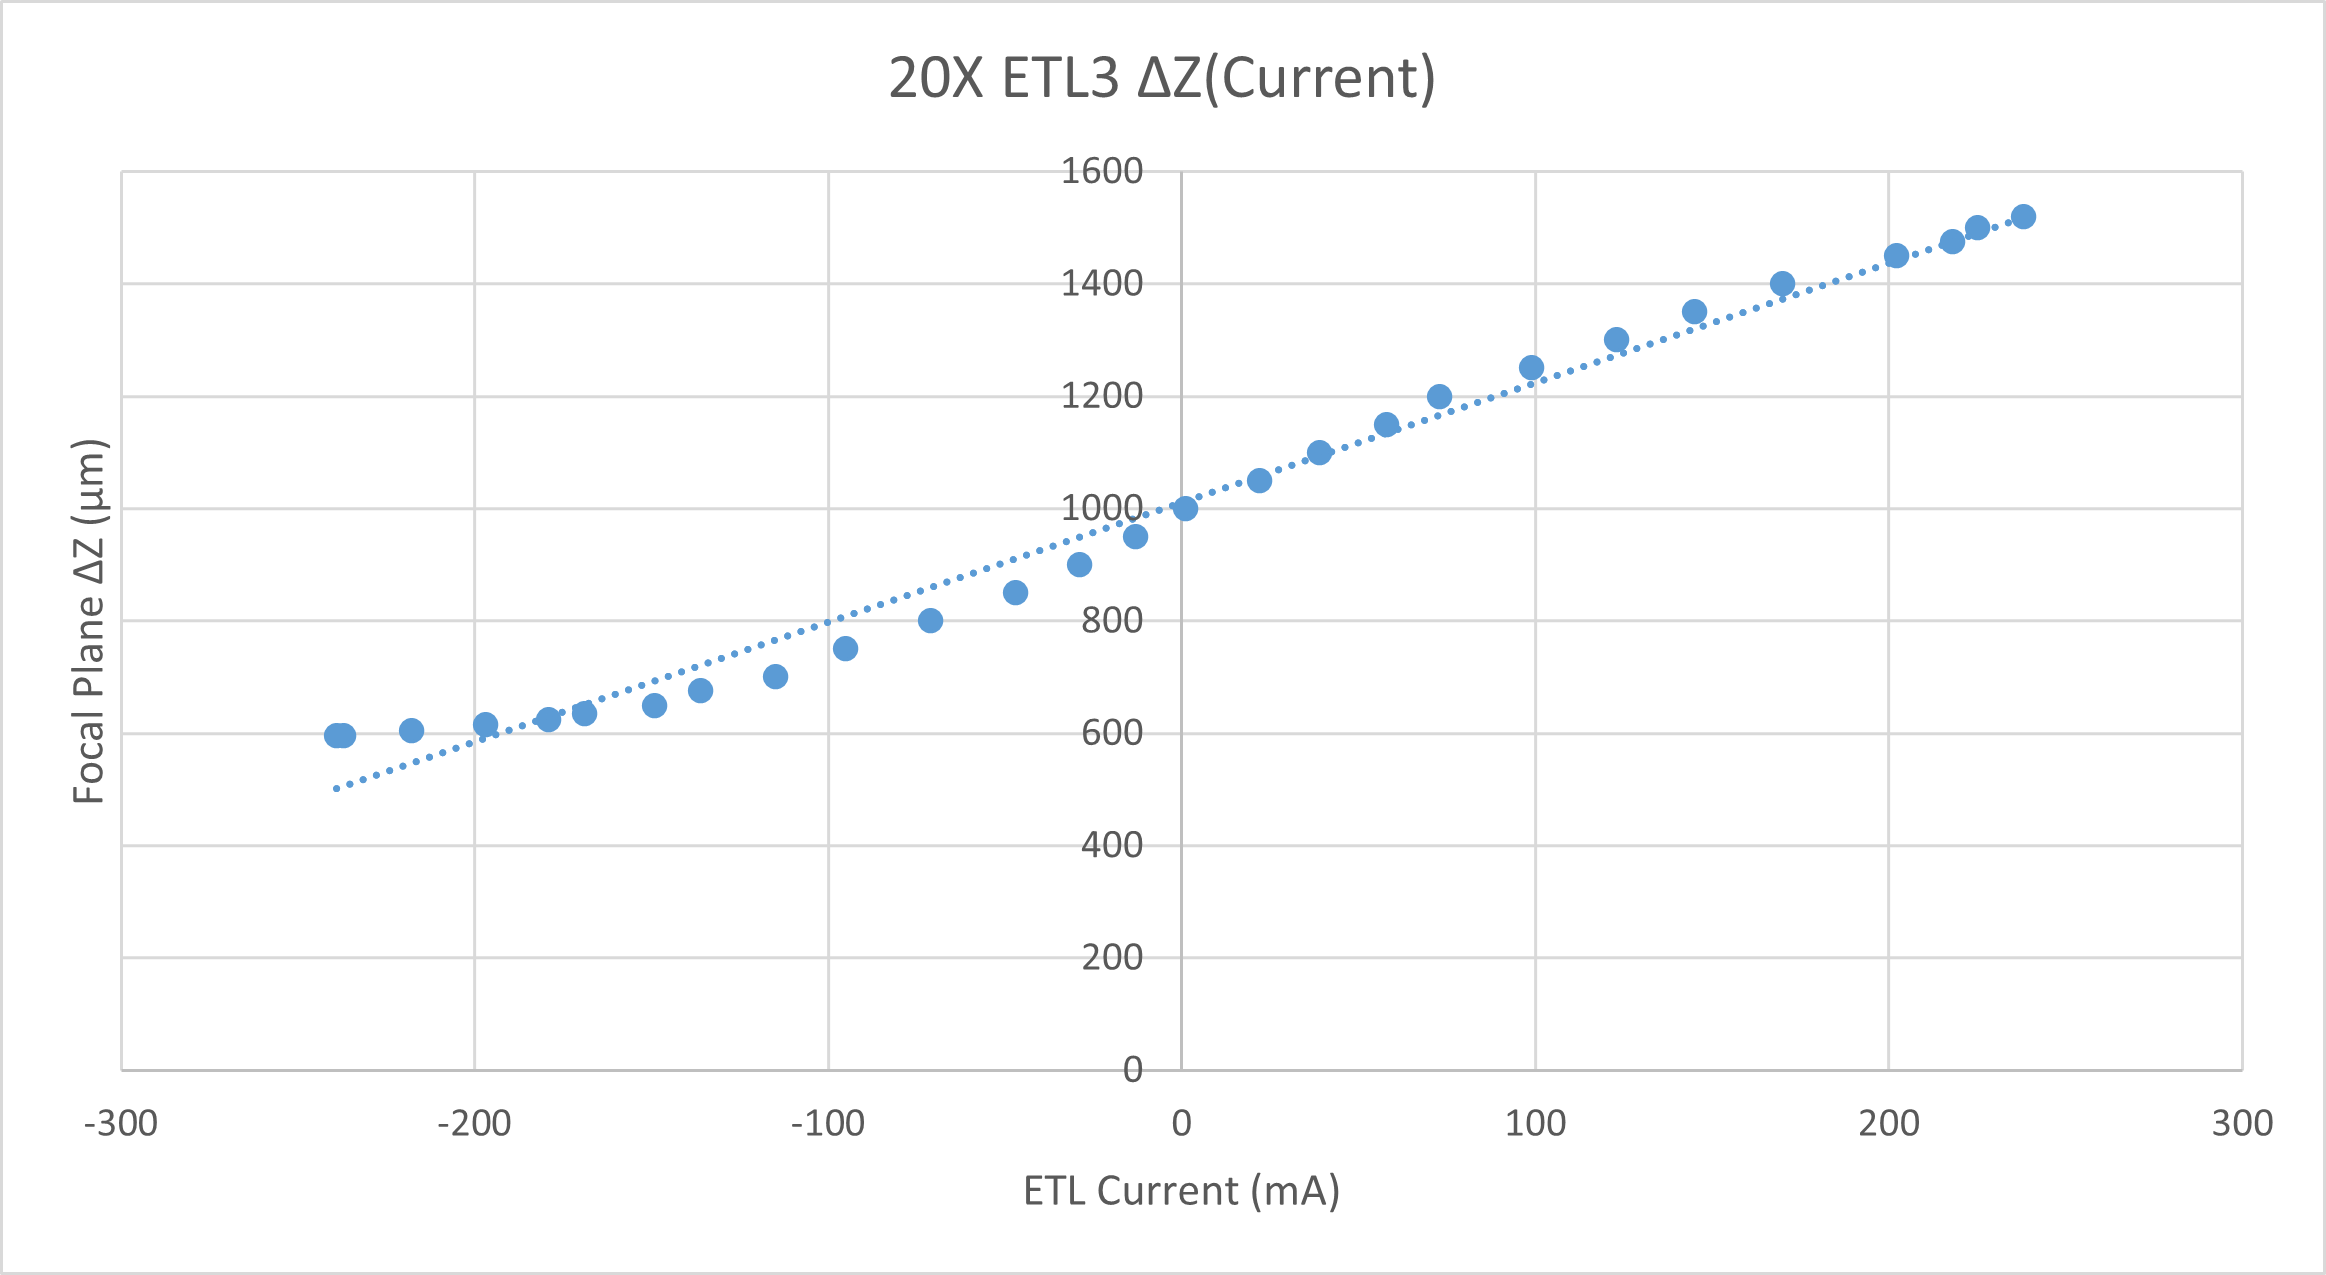
\includegraphics[scale=.75]{20XGraph.png}
    \caption[]{This graph depicts the relationship between ETL3 current and absolute focal plane position. Note the significant breakdown of linearity at large negative currents corresponds to major demagnification and spatial distortion of the image.}
\end{figure}
\begin{figure}
    \centering
    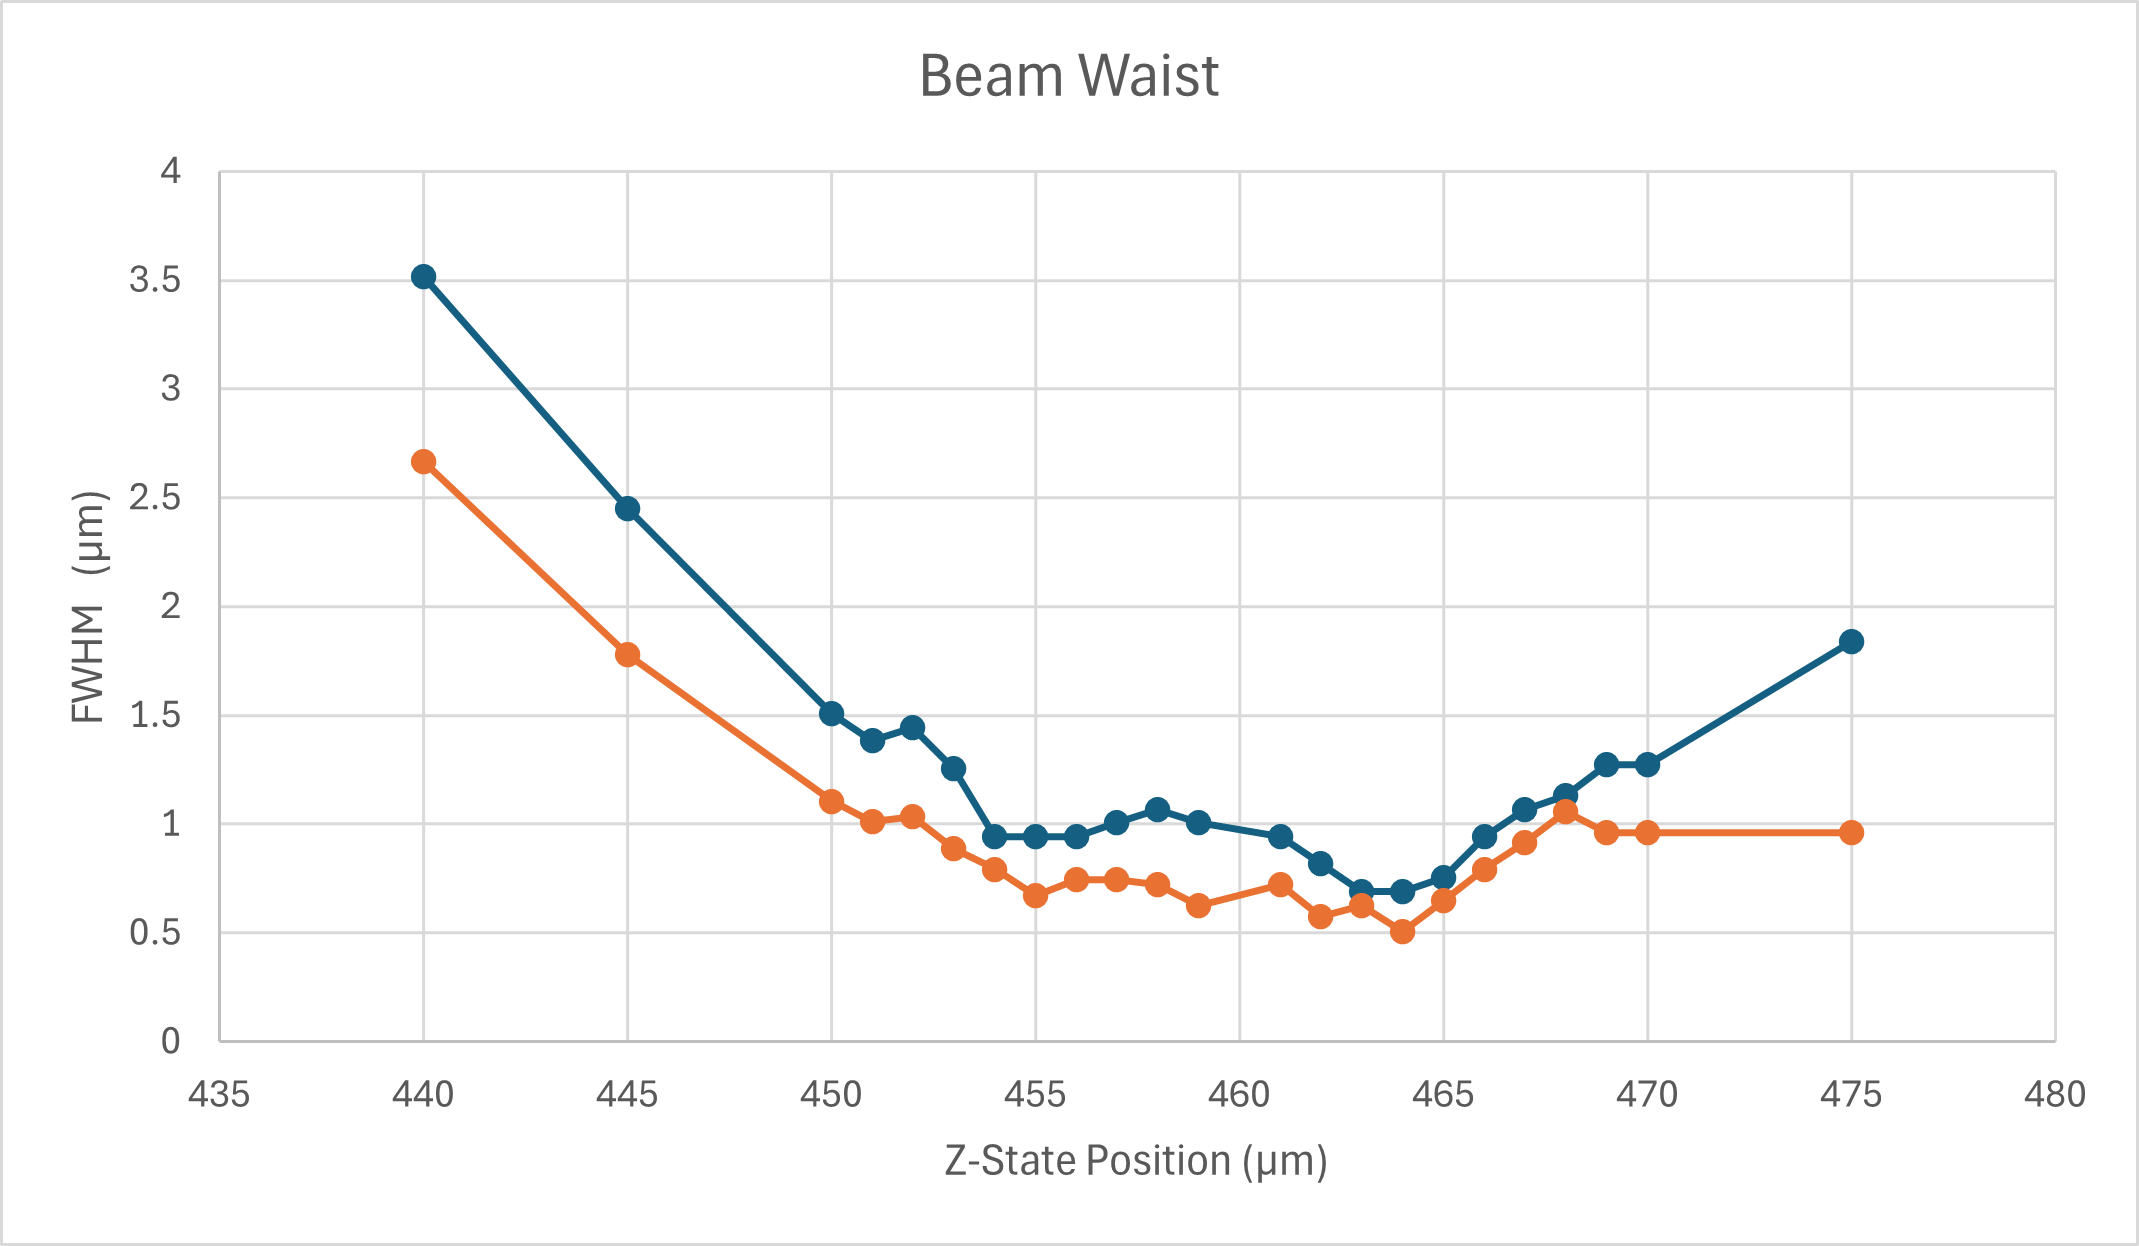
\includegraphics[scale=.75]{BeamWaist.png}
    \caption{This graph depicts the beam waist at a given objective position. The objective used is a 60X Olympus objective. ETL3 was used to keep the beads in focus via remote focusing, allowing us to profile the beam. The red line is the FWHM according to the raw data, while the blue line shows the FWHM of a Gaussian best fit of the data.}
\end{figure}
\begin{figure}
    \centering
    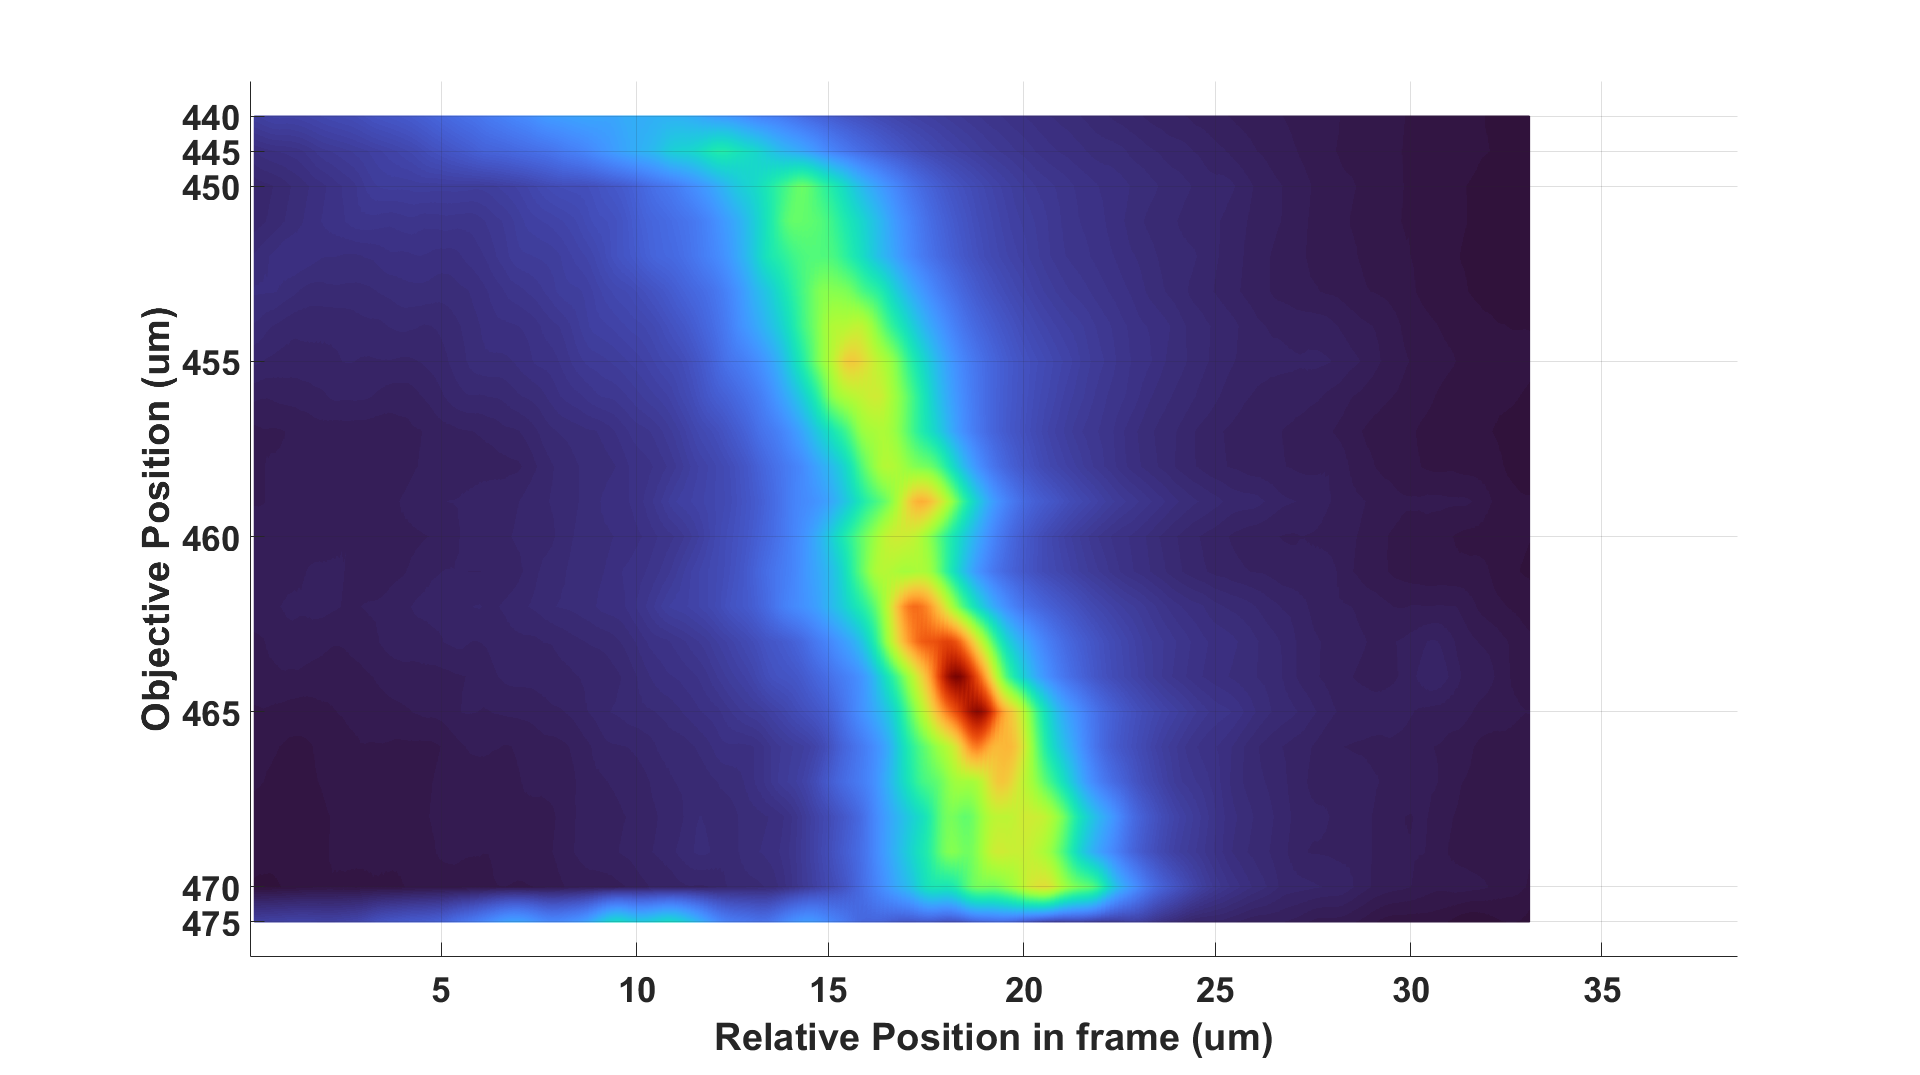
\includegraphics[width=\textwidth]{LS_Heatmap.png}
    \caption{This heatmap displays the intensity of the light sheet as a function of objective's position. Note how the sheet tapers in width and spikes in intensity around the focal plane of the light sheet circa objective position 464 microns. The drift of the light sheet as the objective is translated updwards (down on the graph) shows the lightsheet is emerging at around $75^\circ$, rather than orthogonal to, the sample plane.}
\end{figure}